% Презентация ЛР3 (метод 3: Метрополис — Хастингс для графов).
% Сборка: python scripts/build_lab3_slides.py — пишет lab3_numbers.tex (числа из results/lab3)
% и lab3_fonts.tex, затем компилирует tectonic. Рисунки — выходы ноутбука в results/lab3.
\documentclass[11pt,aspectratio=169]{beamer}
\usepackage{fontspec}
\input{lab3_fonts.tex}
\usepackage{polyglossia}
\setmainlanguage{russian}
\usepackage{amsmath,amssymb}
\usepackage{booktabs}
\usepackage{array}
\usepackage{graphicx}
\graphicspath{{../results/lab3/}}
% Written by scripts/build_lab3_slides.py; do not edit.
\newcommand{\Repeats}{3}
\newcommand{\Alpha}{2}
\newcommand{\Weight}{1}
\newcommand{\SwapShare}{0.3}
\newcommand{\RhoTruthMax}{0.04}
\newcommand{\RlcGraphs}{32}
\newcommand{\RlcDistance}{0.014}
\newcommand{\LostStep}{2}
\newcommand{\BackStep}{108}
\newcommand{\TruthStep}{112}
\newcommand{\RmseMargin}{35}
\newcommand{\RlcShareBefore}{0.746}
\newcommand{\SilicaShareBefore}{0.676}
\newcommand{\WaterShareBefore}{0.505}
\newcommand{\RlcShareAfter}{0.982}
\newcommand{\SilicaShareAfter}{0.968}
\newcommand{\WaterShareAfter}{0.942}
\newcommand{\RhoExtraRlc}{1.28}
\newcommand{\RhoExtraRlcEdge}{R_{m}}
\newcommand{\RhoExtraSilica}{3.12}
\newcommand{\RhoExtraSilicaEdge}{c_{0}}
\newcommand{\RlcSelected}{\{M, R_{2}\}}
\newcommand{\SilicaSelected}{\{a_{1}, a_{2}, a_{3}\}}
\newcommand{\WaterSelected}{\{a_{1}, a_{2}, a_{3}, a_{4}\}}


\definecolor{mred}{RGB}{200,16,46}
\definecolor{mgray}{RGB}{236,236,236}
\usefonttheme[onlymath]{serif}
\setbeamertemplate{navigation symbols}{}
\setbeamercolor{frametitle}{fg=mred,bg=mgray}
\setbeamercolor{title}{fg=mred,bg=mgray}
\setbeamercolor{structure}{fg=mred!80!black}
\setbeamerfont{frametitle}{size=\large}
\setbeamertemplate{frametitle}{%
  \nointerlineskip
  \begin{beamercolorbox}[wd=\paperwidth,ht=3ex,dp=1.4ex,leftskip=0.6em]{frametitle}%
    \usebeamerfont{frametitle}\insertframetitle
  \end{beamercolorbox}}
\setbeamertemplate{footline}{%
  \hfill\usebeamerfont{footline}\scriptsize\insertframenumber\,/\,\inserttotalframenumber\hspace{1em}\vspace{0.8ex}}
\setbeamertemplate{itemize items}[circle]
\setbeamertemplate{enumerate items}[default]
\setbeamersize{text margin left=1.2em,text margin right=1.2em}
\newcommand{\Wone}{W_1}

\title{Метод Метрополиса — Хастингса для графов}
\subtitle{Лабораторная работа 3}
\author{Карпеев Глеб}
\date{2026}

\begin{document}

\begin{frame}[plain]
  \vspace*{-0.4em}
  \begin{beamercolorbox}[wd=\textwidth,sep=0.9em,center]{title}
    {\large\inserttitle}\par\vspace{0.4em}
    {\color{black}\small\insertsubtitle}
  \end{beamercolorbox}
  \vspace{2.2em}
  \centering
  \insertauthor\par\vspace{2.2em}
  \insertdate
\end{frame}

\begin{frame}{Задача}
  Выбрать граф модели семплированием Метрополиса — Хастингса\\
  с учётом интервенции.
  \bigskip

  \begin{tabular}{@{}l@{\quad}l@{}}
    \toprule
    из ЛР1 & модели: два связанных контура; дисперсия кварцевого стекла и воды \\
    из ЛР2 & бутстреп; интервенция — шум в отклике; расстояние Вассерштейна $\Wone$ \\
    новое  & семплер графов, критерий устойчивости ребра и порог, целевая функция \\
    \bottomrule
  \end{tabular}
  \bigskip

  Два этапа: \textbf{без интервенции} $\to$ \textbf{с интервенцией}.
\end{frame}

\begin{frame}{Граф и параметры}
  \centering
  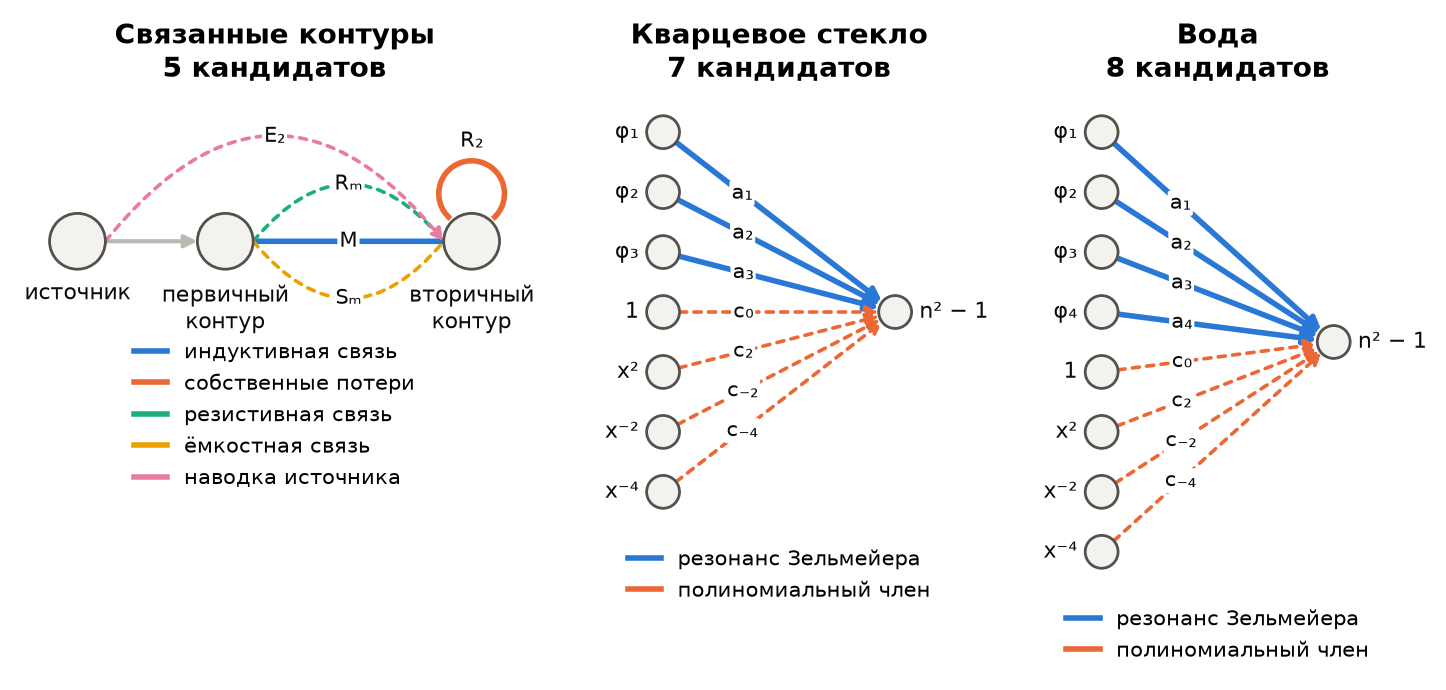
\includegraphics[width=0.70\textwidth]{candidates}

  \begin{tabular}{@{}l@{\quad}l@{}}
    $y=f_G(w,x)$ & модель: $x$ — время или длина волны, $y$ — ток или $n^2-1$ \\
    $G$ & граф: набор рёбер из $K$ кандидатов, $|G|$ — число рёбер \\
    $w_e$ & параметр ребра $e$; без ребра $w_e=w_e^0$ — значение удаления из ЛР2 \\
    & сплошные рёбра порождали данные, пунктирные — лишние
  \end{tabular}
\end{frame}

\begin{frame}{Целевая функция}
  \[
    \pi(G)\propto\exp\bigl(-J(G)\bigr),\qquad
    J(G)=\underbrace{\tfrac12\chi^2(G)}_{\text{невязка}}
    +\tfrac12\ln m\,\Bigl(\underbrace{|G|}_{\text{сложность}}
    +\lambda\underbrace{\textstyle\sum_{e\in G}u_e}_{\text{неустойчивость}}\Bigr)
  \]
  \medskip

  \begin{tabular}{@{}l@{\quad}l@{}}
    $\pi(G)$ & распределение, из которого семплируются графы \\
    $\chi^2(G)$ & взвешенная сумма квадратов остатков после подгонки параметров \\
    $m$ & число наблюдений \\
    $u_e\in[0,1]$ & неустойчивость ребра $e$ к интервенции \\
    $\lambda$ & вес неустойчивости: $0$ без интервенции, $\Weight$ с интервенцией \\
  \end{tabular}
  \bigskip

  \textbf{Порог.} Удаление ребра $e$ выгодно, если $\chi^2$ растёт не более чем на $(1+\lambda u_e)\ln m$.
\end{frame}

\begin{frame}{Критерий устойчивости ребра и порог}
  \vspace{-1.2em}
  \[
    \rho_e=\frac{\overline{\Wone(P_e,P'_e)}}{\Wone(P_e,\delta_{w_e^0})}
    \;\begin{array}{@{}l@{}}
      \leftarrow\text{\small\ сдвиг $w_e$ при интервенции}\\[0.6ex]
      \leftarrow\text{\small\ сдвиг $w_e$ при удалении ребра}
    \end{array}
    \qquad\qquad
    \begin{array}{@{}l@{}}
      u_e=\min(1,\rho_e)\\[0.6ex]
      \text{порог: }\rho_e=1
    \end{array}
  \]
  \vspace{-0.5em}
  {\small
  \begin{tabular}{@{}l@{\quad}l@{}}
    $y'=y+\alpha s(x)\xi$ & интервенция уровня $\alpha$: шум $\xi\sim N(0,1)$, $s(x)$ — масштаб ошибки \\
    $P_e,\ P'_e$ & бутстреп-распределения $w_e$ до и после; черта — среднее по $\Repeats$ шумам $\xi$ \\
    $\delta_{w_e^0}$ & распределение, сосредоточенное в значении удаления $w_e^0$ \\
  \end{tabular}}
  \smallskip

  {\centering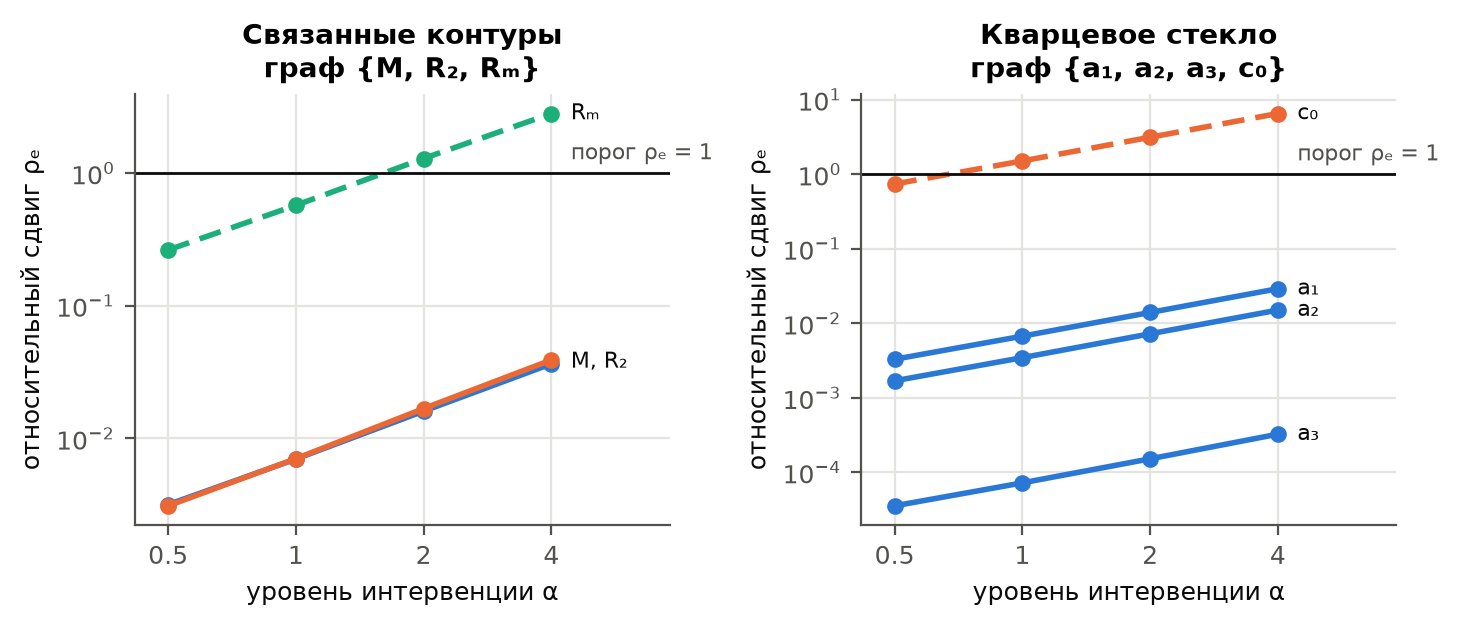
\includegraphics[width=0.58\textwidth]{stability_profile}\par}
  \smallskip

  При $\alpha=\Alpha$: у порождающих рёбер $\rho_e\le\RhoTruthMax$,
  у $\RhoExtraRlcEdge$ — $\RhoExtraRlc$, у $\RhoExtraSilicaEdge$ — $\RhoExtraSilica$.
\end{frame}

\begin{frame}{Алгоритм}
  \begin{columns}[T,onlytextwidth]
    \begin{column}{0.47\textwidth}
      \begin{enumerate}
        \item $G_0$ — полный, пустой или случайный граф.
        \item Предложить $G'\sim Q(\,\cdot\mid G_t)$: добавить или удалить ребро либо,
              с вероятностью $p_s=\SwapShare$, заменить ребро другим.
        \item Принять $G_{t+1}=G'$ с вероятностью $A(G_t,G')$, иначе $G_{t+1}=G_t$.
        \item Выбрать $G^*=\arg\min_t J(G_t)$.
      \end{enumerate}
    \end{column}
    \begin{column}{0.50\textwidth}
      \textbf{Переработка structure MCMC}
      \smallskip

      \small
      \begin{tabular}{@{}l>{\raggedright\arraybackslash}p{0.26\linewidth}>{\raggedright\arraybackslash}p{0.40\linewidth}@{}}
        \toprule
        & было & стало \\
        \midrule
        ход & обратить ребро & заменить ребро другим \\
        \addlinespace
        цель & $p(G\mid y)$ & $\exp(-J(G))$ \\
        \addlinespace
        удаление & равномерно & с весом $v_e=\varepsilon+u_e$, $\varepsilon>0$ \\
        \bottomrule
      \end{tabular}
    \end{column}
  \end{columns}
  \medskip
  \[
    A(G_t,G')=\min\Bigl\{1,\ \exp\bigl(J(G_t)-J(G')\bigr)\,\frac{Q(G_t\mid G')}{Q(G'\mid G_t)}\Bigr\}
  \]
\end{frame}

\begin{frame}{Корректность}
  \begin{tabular}{@{}l@{\quad}l@{}}
    \toprule
    обратимость & $\pi(G)\,Q(G'\mid G)\,A(G,G')$ симметрично по $G$ и $G'$ \\
    неприводимость & $v_e>0$: между любыми графами не более $K$ ходов \\
    апериодичность & в пустом и полном графе ход замены оставляет цепь на месте \\
    \bottomrule
  \end{tabular}
  \smallskip

  $\Rightarrow$ при любом $G_0$ частоты графов в цепи сходятся к $\pi(G)$.

  \begin{center}
    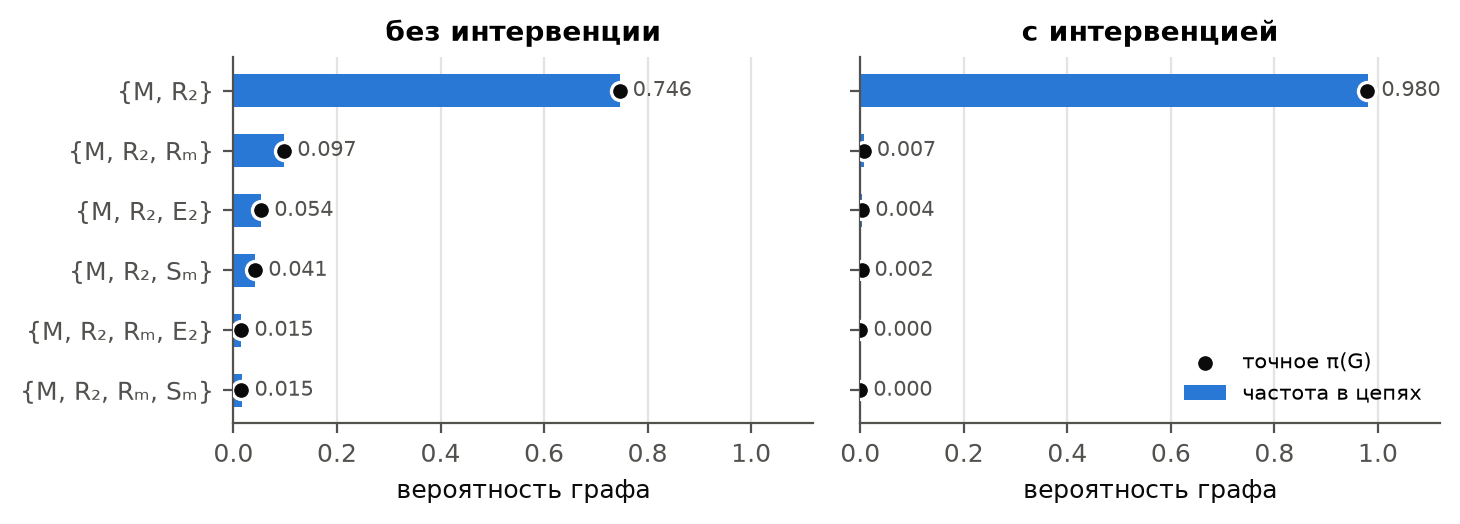
\includegraphics[width=0.68\textwidth]{rlc_posterior}
  \end{center}
  \vspace{-0.7em}
  Перебор $\RlcGraphs$ графов: полная вариация между частотами в цепях и $\pi$ не больше $\RlcDistance$.
\end{frame}

\begin{frame}{Последовательность семплированных графов}
  \centering
  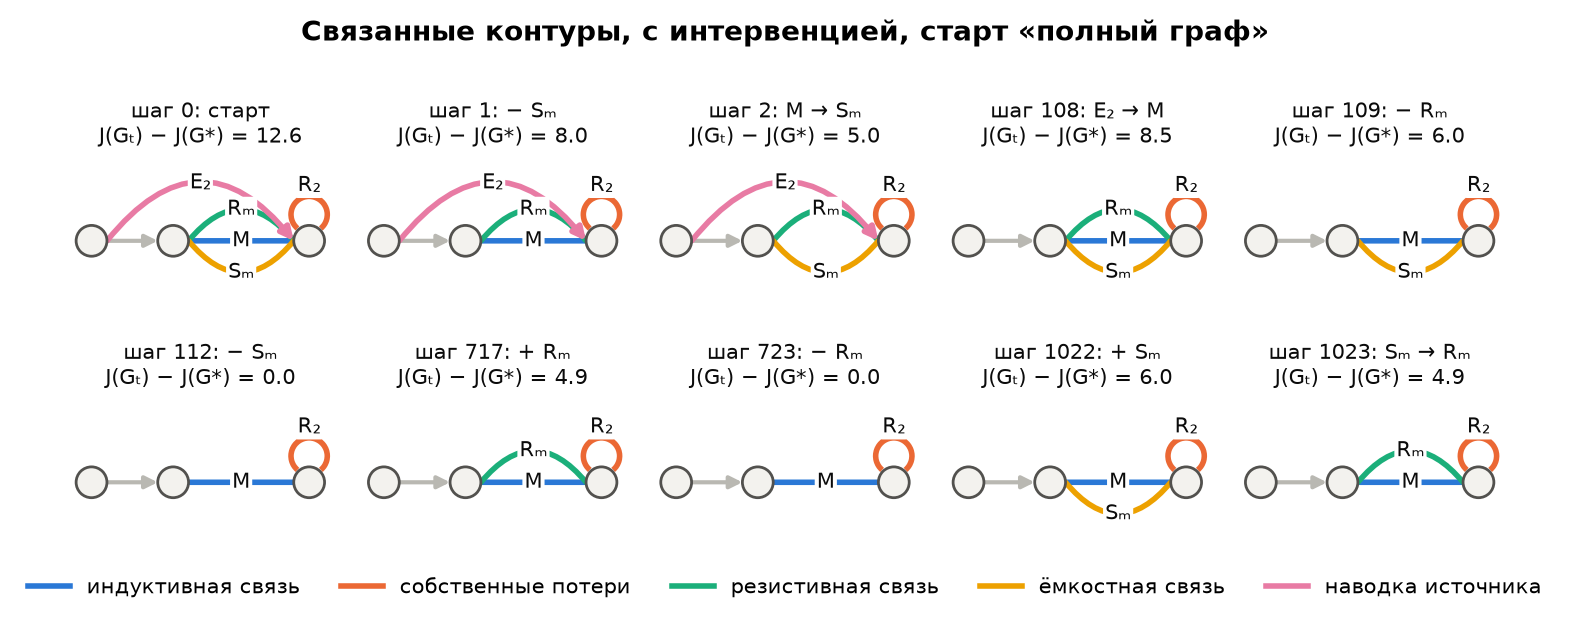
\includegraphics[width=0.92\textwidth]{rlc_sequence}
  \medskip

  Цепь теряет $M$ на шаге $\LostStep$, возвращает его заменой на шаге $\BackStep$\\
  и приходит в $\RlcSelected$ на шаге $\TruthStep$.
\end{frame}

\begin{frame}{Выбор графа}
  \textbf{На обоих этапах выбран порождающий граф.}
  \smallskip

  \centering
  {\small
  \begin{tabular}{@{}lccc@{}}
    \toprule
    & контуры & кварцевое стекло & вода \\
    \midrule
    выбранный граф $G^*$ & $\RlcSelected$ & $\SilicaSelected$ & $\WaterSelected$ \\
    \addlinespace
    частота $G^*$ в цепях \\
    \quad без интервенции & $\RlcShareBefore$ & $\SilicaShareBefore$ & $\WaterShareBefore$ \\
    \quad с интервенцией & $\RlcShareAfter$ & $\SilicaShareAfter$ & $\WaterShareAfter$ \\
    \bottomrule
  \end{tabular}}

  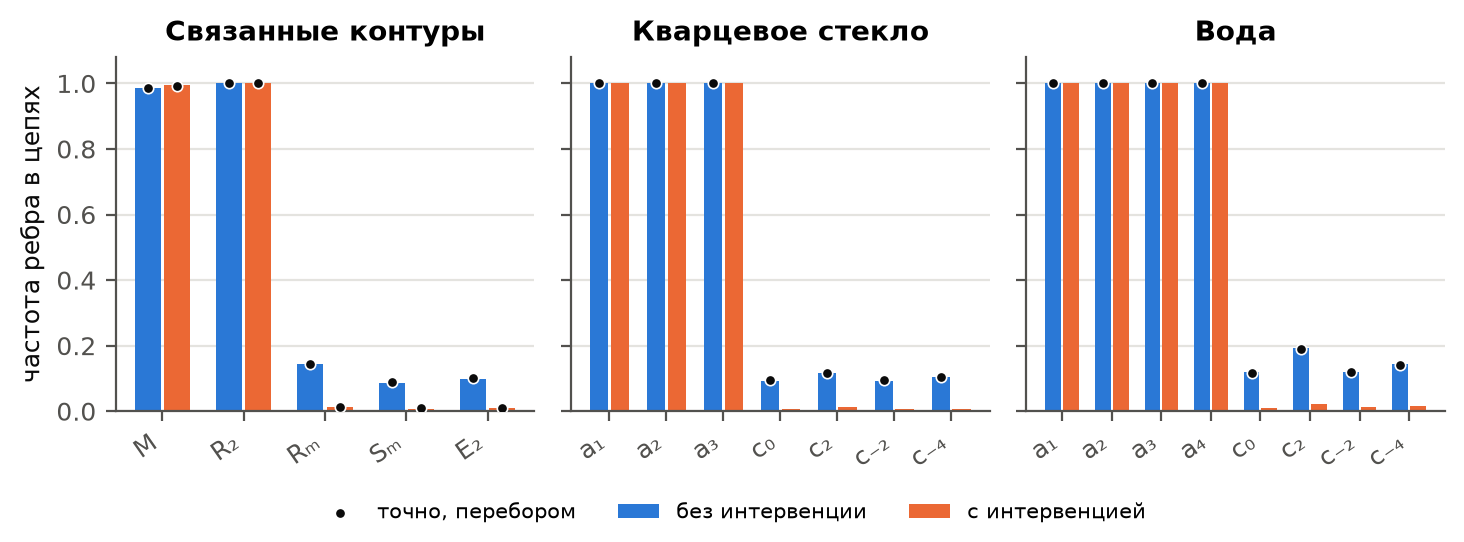
\includegraphics[width=0.62\textwidth]{edge_frequencies}

  \raggedright
  \textbf{С интервенцией лишние рёбра встречаются примерно на порядок реже.}
\end{frame}

\begin{frame}{Выборка и аппроксимация выбранным графом}
  \begin{columns}[c,onlytextwidth]
    \begin{column}{0.58\textwidth}
      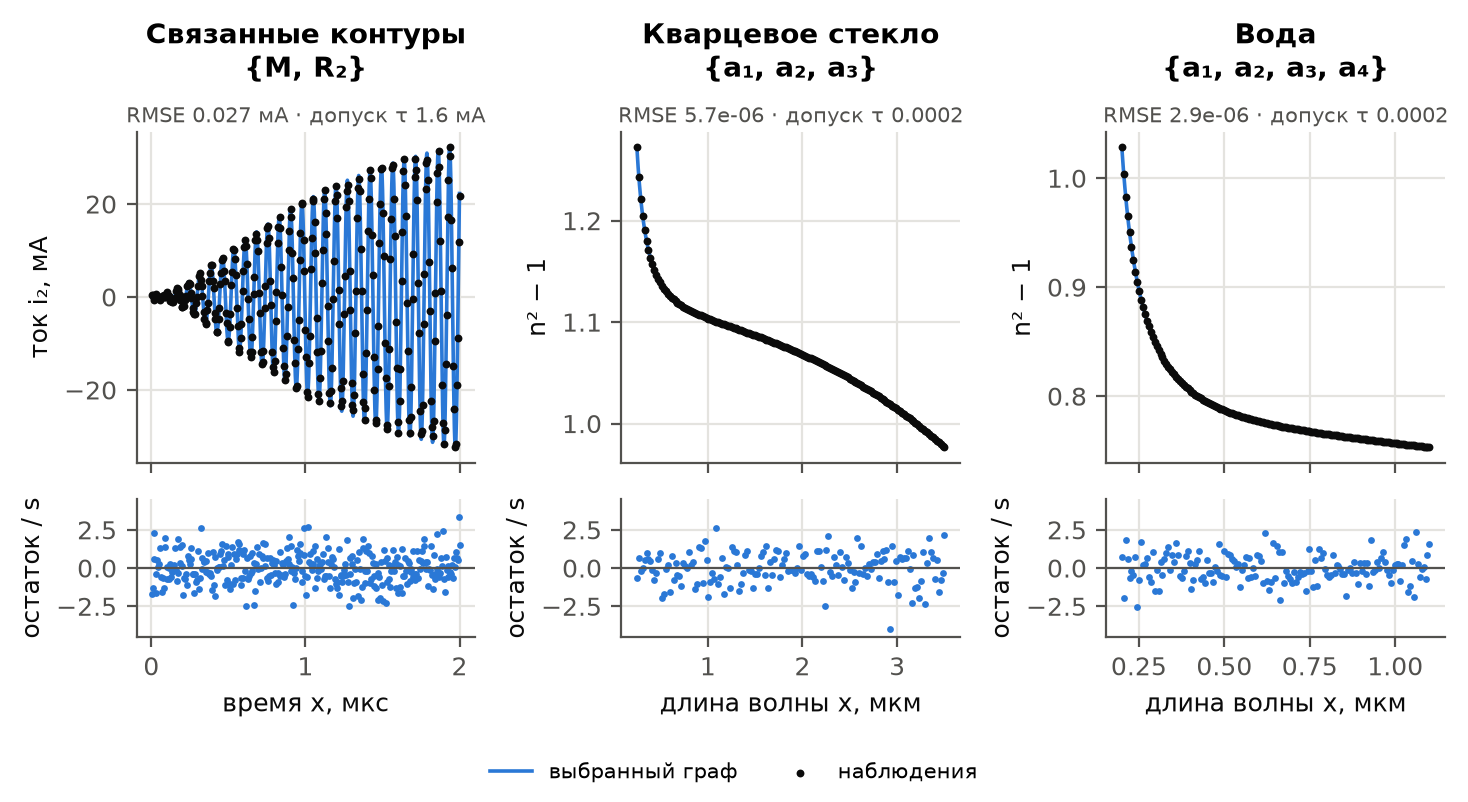
\includegraphics[width=\textwidth]{approximation}
    \end{column}
    \begin{column}{0.39\textwidth}
      \raggedright
      \textbf{Итоги}
      \begin{itemize}
        \item RMSE на отложенной сетке меньше допуска $\tau$ в~$\RmseMargin$ раз и более.
        \item Выбор графа интервенция не меняет: лишние рёбра проигрывают и без неё.
        \item Шум в отклике не проверяет направление связи.
      \end{itemize}
    \end{column}
  \end{columns}
\end{frame}

\end{document}
